\documentclass[10]{article}
%\documentclass[11pt]{article}
\usepackage{hyperref}
\usepackage{amsfonts,amssymb,amsmath,amsthm,cite}
\usepackage{graphicx}
\usepackage[toc,page]{appendix}
\usepackage{nicefrac}
%% \usepackage[francais]{babel}
\usepackage[applemac]{inputenc}
\usepackage{amssymb, euscript}
\usepackage[matrix,arrow,curve]{xy}
\usepackage{graphicx}
\usepackage{tabularx}
\usepackage{float}
\usepackage{tikz}
\usepackage{slashed}
\usepackage{mathrsfs}
\usepackage{multirow}
\usepackage{rotating}
\usepackage{mathbbol}

%\usepackage{mathtools}

\usetikzlibrary{matrix}
\usetikzlibrary{cd}

\usepackage{siunitx}

\usepackage{lmodern}
\usepackage[T1]{fontenc}
\usepackage[babel=true]{microtype}


\usepackage{amsfonts,cite}
\usepackage{graphicx}

%% \usepackage[francais]{babel}
\usepackage[applemac]{inputenc}


\usepackage[sc]{mathpazo}
\usepackage{environ}

\linespread{1.05}         % Palatino needs more leading (space between lines)


%\usepackage[usenames]{color}



\DeclareFontFamily{T1}{pzc}{}
\DeclareFontShape{T1}{pzc}{m}{it}{1.8 <-> pzcmi8t}{}
\DeclareMathAlphabet{\mathpzc}{T1}{pzc}{m}{it}
% the command for it is \mathpzc

\textwidth=140mm


% % % % % % % % % % % % % % % % % % % %
\theoremstyle{plain}
\newtheorem{prop}{Proposition}[section]
\newtheorem{prdf}[prop]{Proposition and Definition}
\newtheorem{lem}[prop]{Lemma}%[section]
\newtheorem{cor}[prop]{Corollary}%[section]
\newtheorem{thm}[prop]{Theorem}%[section]
\newtheorem{theorem}[prop]{Theorem}
\newtheorem{lemma}[prop]{Lemma}
\newtheorem{proposition}[prop]{Proposition}
\newtheorem{corollary}[prop]{Corollary}
\newtheorem{statement}[prop]{Statement}

\theoremstyle{definition}
\newtheorem{defn}[prop]{Definition}%[section]
\newtheorem{cordefn}[prop]{Corollary and Definition}%[section]
\newtheorem{empt}[prop]{}%[section]
\newtheorem{exm}[prop]{Example}%[section]
\newtheorem{rem}[prop]{Remark}%[section]
\newtheorem{prob}[prop]{Problem}
\newtheorem{conj}{Conjecture}       %% Hypothesis 1
\newtheorem{cond}{Condition}        %% Condition 1
%\newtheorem{axiom}[thm]{Axiom}           %% Axiom 1 modified
\newtheorem{fact}[prop]{Fact}
\newtheorem{ques}{Question}         %% Question 1
\newtheorem{answ}{Answer}           %% Answer 1
\newtheorem{notn}{Notation}        %% Notations are not numbered

\theoremstyle{definition}
\newtheorem{notation}[prop]{Notation}
\newtheorem{definition}[prop]{Definition}
\newtheorem{example}[prop]{Example}
\newtheorem{exercise}[prop]{Exercise}
\newtheorem{conclusion}[prop]{Conclusion}
\newtheorem{conjecture}[prop]{Conjecture}
\newtheorem{criterion}[prop]{Criterion}
\newtheorem{summary}[prop]{Summary}
\newtheorem{axiom}[prop]{Axiom}
\newtheorem{problem}[prop]{Problem}
%\theoremstyle{remark}
\newtheorem{remark}[prop]{Remark}

\numberwithin{equation}{section}
\newtheorem*{claim}{Claim}
\DeclareMathOperator{\Dom}{Dom}              %% domain of an operator
\newcommand{\Dslash}{{D\mkern-11.5mu/\,}}    %% Dirac operator
\newcommand{\trG}{{\rm tr}_G\;}
\newcommand{\trF}{{\rm tr}_{\cal F}\;}
\newcommand{\TR}{{\rm TR}\;}
\newcommand{\res}{{\rm res}\;}


\newcommand\ci{${\mathcal C}^{\infty}$}
\newcommand\CI{{\mathcal C}^{\infty}}
\newcommand\CIc{{\mathcal C}^{\infty}_{\text{c}}}

%\newcommand\myeq{\stackrel{\mathclap{\normalfont\mbox{def}}}{=}}
\newcommand{\rar}[1]{\stackrel{#1}{\longrightarrow}}
\newcommand{\lar}[1]{\stackrel{#1}{\longleftarrow}}

\newcommand{\nor}[1]{\left\Vert #1\right\Vert}    %\nor{x}=||x||
\newcommand{\norm}[1]{\left\| #1\right\|}    %\nor{x}=||x||
\newcommand{\vertiii}[1]{{\left\vert\kern-0.25ex\left\vert\kern-0.25ex\left\vert #1
		\right\vert\kern-0.25ex\right\vert\kern-0.25ex\right\vert}}
\newcommand{\Ga}{\Gamma}  
\newcommand{\coker}{\mathrm{coker}}                   %% short for  \Gamma
\newcommand{\Coo}{C^\infty}                  %% smooth functions
\newcommand{\dom}{\mathrm{dom}}                  %% smooth functions
\newcommand{\Cont}{C} 
\newcommand{\cl}{\overline} 
\newcommand{\Contc}{C_c} 
\newcommand{\Contb}{C_b} 
\newcommand{\Repi}{\mathrm{Rep}_{int}} 
\newcommand{\Rep}{\mathrm{Rep}} 
\newcommand{\hor}[0]{\mathrm{hor}}
\newcommand{\comp}{\operatorname{comp}}
\newcommand{\adb}{\operatorname{adb}}
\newcommand{\dist}{\operatorname{dist}}


% % % % % % % % % % % % % % % % % % % %


\usepackage[sc]{mathpazo}
\linespread{1.05}         % Palatino needs more leading (space between lines)

\newbox\ncintdbox \newbox\ncinttbox %% noncommutative integral symbols
\setbox0=\hbox{$-$} \setbox2=\hbox{$\displaystyle\int$}
\setbox\ncintdbox=\hbox{\rlap{\hbox
		to \wd2{\hskip-.125em \box2\relax\hfil}}\box0\kern.1em}
\setbox0=\hbox{$\vcenter{\hrule width 4pt}$}
\setbox2=\hbox{$\textstyle\int$} \setbox\ncinttbox=\hbox{\rlap{\hbox
		to \wd2{\hskip-.175em \box2\relax\hfil}}\box0\kern.1em}

\newcommand{\ncint}{\mathop{\mathchoice{\copy\ncintdbox}%
		{\copy\ncinttbox}{\copy\ncinttbox}%
		{\copy\ncinttbox}}\nolimits}  %% NC integral

%%% Repeated relations:
\newcommand{\xyx}{\times\cdots\times}      %% repeated product
\newcommand{\opyop}{\oplus\cdots\oplus}    %% repeated direct sum
\newcommand{\oxyox}{\otimes\cdots\otimes}  %% repeated tensor product
\newcommand{\wyw}{\wedge\cdots\wedge}      %% repeated exterior product
\newcommand{\subysub}{\subset\hdots\subset}      %% repeated subset
\newcommand{\supysup}{\supset\hdots\supset}      %% repeated supset
\newcommand\CC{\mathbb C}
\newcommand\NN{\mathbb N}
\newcommand\RR{\mathbb R}
\newcommand\ZZ{\mathbb Z}
\newcommand{\LGR}{\matcal L}
\newcommand{\rep}{\mathfrak{rep}}
\newcommand{\lift}{\mathfrak{lift}}
\newcommand{\desc}{\mathfrak{desc}}
\newcommand{\Cstar}{C^*}
\newcommand{\Cst}{C^*}
\newcommand{\Star}{*}
\newcommand{\PS}[1]{\Psi^{#1}(\GR;E)}

%%% Roman letters:
\newcommand{\id}{\mathrm{id}}                %% identity map
\newcommand{\Id}{\mathrm{Id}}                %% identity map
\newcommand{\pt}{\mathrm{pt ???}}                %% a point
\newcommand{\const}{\mathrm{const}}          %% a constant
\newcommand{\codim}{\mathrm{codim}}          %% codimension
\newcommand{\cyc}{\mathrm{cyclic}}  %% cyclic sum
\renewcommand{\d}{\mathrm{d}}       %% commutative differential
\newcommand{\dR}{\mathrm{dR}}       %% de~Rham cohomology
\newcommand{\proj}{\mathrm{proj}}                %% a projection
\newcommand*{\braket}[2]{\langle#1 {,~} #2\rangle}% right inner products
\newcommand*{\lbraket}[2]{\langle\!\langle#1{\mid}#2\rangle\!\rangle}% left inner products

\newcommand*{\Mult}{\mathcal M}% multiplier algebra
\newcommand{\Lt}{\mathcal{L}}                 %%\newcommand{\unitsv}[1]{#1^{(0)}}

\newcommand{\A}{\mathcal{A}}                 %%\newcommand{\unitsv}[1]{#1^{(0)}}
\newcommand{\units}{G^{(0)}}
\newcommand{\haars}{\{\lambda^{u}\}_{u\in\units}}
\newcommand{\shaars}{\{\lambda_{u}\}_{u\in\units}}
\newcommand{\haarsv}[2]{\{\lambda^{#2}_{#1}\}_{#2\in\unitsv{#1}}}
\newcommand{\haarv}[2]{\lambda^{#2}_{#1}}

\renewcommand{\a}{\alpha}                    %% short for  \alphapha
\DeclareMathOperator{\ad}{ad}                %% infml adjoint repn
\newcommand{\as}{\quad\mbox{as}\enspace}     %% `as' with spacing
\newcommand{\Aun}{\widetilde{\mathcal{A}}}   %% unital algebra
\newcommand{\B}{\mathcal{B}}                 %% space of distributions
\newcommand{\E}{\mathcal{E}}                 %% space of distributions
\renewcommand{\b}{\beta}                     %% short for \beta
\newcommand{\braCket}[3]{\langle#1\mathbin|#2\mathbin|#3\rangle}
%\newcommand{\braket}[2]{\langle#1\mathbin|#2\rangle} %% <w|z>
\newcommand{\C}{\mathbb{C}}                  %% complex numbers
\newcommand{\cc}{\mathbf{c}}                 %% Hochschild cycle
\DeclareMathOperator{\Cl}{C\ell}             %% Clifford algebra
\newcommand{\F}{\mathcal{F}}                 %% space of test functions
\newcommand{\G}{\mathcal{G}}                 %% 
\newcommand{\GR}{\mathcal{G}}                 %% 
\newcommand{\D}{\mathcal{D}}                 %% Moyal L^2-filtration
\renewcommand{\H}{\mathcal{H}}               %% Hilbert space
\newcommand{\half}{\tfrac{1}{2}}             %% small fraction  1/2
\newcommand{\hh}{\mathcal{H}}                %% Hilbert space
\newcommand{\hookto}{\hookrightarrow}        %% abbreviation
\newcommand{\Ht}{{\widetilde{\mathcal{H}}}}  %% Hilbert space of forms
\newcommand{\I}{\mathcal{I}}                 %% tracelike functions
\DeclareMathOperator{\Junk}{Junk}            %% the junk DGA ideal
\newcommand{\K}{\mathcal{K}}                 %% compact operators
\newcommand{\ket}[1]{|#1\rangle}             %% ket vector
\newcommand{\ketbra}[2]{|#1\rangle\langle#2|} %% rank one operator
\renewcommand{\L}{\mathcal{L}}               %% operator algebra
\newcommand{\La}{\Lambda}                    %% short for \Lambda
\newcommand{\la}{\lambda}                    %% short for \lambda
\newcommand{\lf}{L_f^\theta}                 %% left  mult operator
\newcommand{\M}{\mathcal{M}}                 %% Moyal multplr algebra
\newcommand{\Lb}{\mathcal{L}}                 %% Moyal multplr algebra
\newcommand{\mm}{\mathcal{M}^\theta}
%\newcommand{{{\star_{\theta}}}{{\mathchoice{\mathbin{\;|\;ar_{_\theta}}}
			%            {\mathbin{\;|\;ar_{_\theta}}}           %% Moyal
			%            {{\;|\;ar_\theta}}{{\;|\;ar_\theta}}}}    %% product
	\newcommand{\N}{\mathbb{N}}                  %%  integers
	\newcommand{\nb}{\nabla}                     %% gradient
	\newcommand{\Oh}{\mathcal{O}}                %% comm multiplier alg
	\newcommand{\om}{\omega}                     %% short for \omega
	\newcommand{\opp}{{\mathrm{op}}}             %% opposite algebra
	\newcommand{\ox}{\otimes}                    %% tensor product
	\newcommand{\eps}{\varepsilon}                    %% tensor product
	\newcommand{\otimesyox}{\otimes\cdots\otimes}    %% repeated tensor product
	\newcommand{\pa}{\partial}                   %% short for \partial
	\newcommand{\pd}[2]{\frac{\partial#1}{\partial#2}}%% partial derivative
	\newcommand{\piso}[1]{\lfloor#1\rfloor}      %% integer part
	\newcommand{\PsiDO}{\Psi~\mathrm{DO}}         %% pseudodiffl operators
	\newcommand{\Q}{\mathbb{Q}}                  %% rational numbers
	\newcommand{\R}{\mathbb{R}}                  %% real numbers
	\newcommand{\rdl}{R_\Dslash(\lambda)}        %% resolvent
	\newcommand{\roundbraket}[2]{(#1\mathbin|#2)} %% (w|z)
	\newcommand{\row}[3]{{#1}_{#2},\dots,{#1}_{#3}} %% list: a_1,...,a_n
	\newcommand{\sepword}[1]{\quad\mbox{#1}\quad} %% well-spaced words
	\newcommand{\set}[1]{\{\,#1\,\}}             %% set notation
	\newcommand{\Sf}{\mathbb{S}}                 %% sphere
	\newcommand{\uhor}[1]{\Omega^1_{hor}#1}
	\newcommand{\sco}[1]{{\sp{(#1)}}}
	\newcommand{\sw}[1]{{\sb{(#1)}}}
	\DeclareMathOperator{\spec}{sp}              %% spectrum
	\renewcommand{\SS}{\mathcal{S}}              %% Schwartz space
	\newcommand{\sss}{\mathcal{S}}               %% Schwartz space
	\DeclareMathOperator{\supp}{\mathfrak{supp}}            %% support
	\newcommand{\T}{\mathbb{T}}                  %% circle as a group
	\renewcommand{\th}{\theta}                   %% short for \theta
	\newcommand{\thalf}{\tfrac{1}{2}}            %% small* fraction 1/2
	\newcommand{\tihalf}{\tfrac{i}{2}}           %% small* fraction i/2
	\newcommand{\tpi}{{\tilde\pi}}               %% extended representation
	\DeclareMathOperator{\Tr}{Tr}                %% trace of operator
	\DeclareMathOperator{\tr}{tr}                %% trace of matrix
	\newcommand{\del}{\partial}                  %% short for  \partial
	\DeclareMathOperator{\tsum}{{\textstyle\sum}} %% small sum in display
	\newcommand{\V}{\mathcal{V}}                 %% test function space
	\newcommand{\vac}{\ket{0}}                   %% vacuum ket vector
	\newcommand{\vf}{\varphi}                    %% scalar field
	\newcommand{\w}{\wedge}                      %% exterior product
	\DeclareMathOperator{\wres}{wres}            %% density of Wresidue
	\newcommand{\x}{\times}                      %% cross
	\newcommand{\Z}{\mathbb{Z}}                  %% integers
	\newcommand{\7}{\dagger}                     %% short for + symbol
	\newcommand{\8}{\bullet}                     %% anonymous degree
	\renewcommand{\.}{\cdot}                     %% anonymous variable
	\renewcommand{\:}{\colon}                    %% colon in  f: A -> B
	
	%\newcommand{\sA}{\mathscr{A}}       %%
	\newcommand{\sA}{\mathcal{A}} 
	\newcommand{\sB}{\mathcal{B}}       %%
	\newcommand{\sC}{\mathcal{C}}       %%
	\newcommand{\sD}{\mathcal{D}}       %%
	\newcommand{\sE}{\mathcal{E}}       %%
	\newcommand{\sF}{\mathcal{F}}       %%
	\newcommand{\sG}{\mathcal{G}}       %%
	\newcommand{\sH}{\mathcal{H}}       %%
	\newcommand{\sI}{\mathcal{I}}       %%
	\newcommand{\sJ}{\mathcal{J}}       %%
	\newcommand{\sK}{\mathcal{K}}       %%
	\newcommand{\sL}{\mathcal{L}}       %%
	\newcommand{\sM}{\mathcal{M}}       %%
	\newcommand{\sN}{\mathcal{N}}       %%
	\newcommand{\sO}{\mathcal{O}}       %%
	\newcommand{\sP}{\mathcal{P}}       %%
	\newcommand{\sQ}{\mathcal{Q}}       %%
	\newcommand{\sR}{\mathcal{R}}       %%
	\newcommand{\sS}{\mathcal{S}}       %%
	\newcommand{\sT}{\mathcal{T}}       %%
	\newcommand{\sU}{\mathcal{U}}       %%
	\newcommand{\sV}{\mathcal{V}}       %%
	\newcommand{\sX}{\mathcal{X}}       %%
	\newcommand{\sY}{\mathcal{Y}}       %%
	\newcommand{\sZ}{\mathcal{Z}}       %%
	
	\newcommand{\Om}{\Omega}       %%
	
	
	\DeclareMathOperator{\ptr}{ptr}     %% Poisson trace
	\DeclareMathOperator{\Trw}{Tr_\omega} %% Dixmier trace
	\DeclareMathOperator{\vol}{Vol}     %% total volume
	\DeclareMathOperator{\Vol}{Vol}     %% total volume
	\DeclareMathOperator{\Area}{Area}   %% area of a surface
	\DeclareMathOperator{\Wres}{Wres}   %% (Wodzicki) residue
	
	\newcommand{\dd}[1]{\frac{\partial}{\partial#1}}   %% partial derivation
	\newcommand{\ddt}[1]{\frac{d}{d#1}}                %% derivative
	\newcommand{\inv}[1]{\frac{1}{#1}}                 %% inverse
	\newcommand{\sfrac}[2]{{\scriptstyle\frac{#1}{#2}}} %% tiny fraction
	
	\newcommand\VD{{\mathcal D}}
	\newcommand{\bA}{\mathbb{A}}       %%
	\newcommand{\bB}{\mathbb{B}}       %%
	\newcommand{\bC}{\mathbb{C}}       %%
	\newcommand{\bCP}{\mathbb{C}P}     %%
	\newcommand{\bD}{\mathbb{D}}       %%
	\newcommand{\bE}{\mathbb{E}}       %%
	\newcommand{\bF}{\mathbb{F}}       %%
	\newcommand{\bG}{\mathbb{G}}       %%
	\newcommand{\bH}{\mathbb{H}}       %%
	\newcommand{\bHP}{\mathbb{H}P}     %%
	\newcommand{\bI}{\mathbb{I}}       %%
	\newcommand{\bJ}{\mathbb{J}}       %%
	\newcommand{\bK}{\mathbb{K}}       %%
	\newcommand{\bL}{\mathbb{L}}       %%
	\newcommand{\bM}{\mathbb{M}}       %%
	\newcommand{\bN}{\mathbb{N}}       %%
	\newcommand{\bO}{\mathbb{O}}       %%
	\newcommand{\bOP}{\mathbb{O}P}     %%
	\newcommand{\bP}{\mathbb{P}}       %%
	\newcommand{\bQ}{\mathbb{Q}}       %%
	\newcommand{\bR}{\mathbb{R}}       %%
	\newcommand{\bRP}{\mathbb{R}P}     %%
	\newcommand{\bS}{\mathbb{S}}       %%
	\newcommand{\bT}{\mathbb{T}}       %%
	\newcommand{\bU}{\mathbb{U}}       %%
	\newcommand{\bV}{\mathbb{V}}       %%
	\newcommand{\bX}{\mathbb{X}}       %%
	\newcommand{\bY}{\mathbb{Y}}       %%
	\newcommand{\bZ}{\mathbb{Z}}       %%
	
	\newcommand{\bydef}{\stackrel{\mathrm{def}}{=}}          %% 
	\newcommand{\defeq}{\stackrel{\mathrm{def}}{=}}   
	
	
	
	\newcommand{\al}{\alpha}          %% short for  \alpha
	\newcommand{\bt}{\beta}           %% short for  \beta
	\newcommand{\Dl}{\Delta}          %% short for  \Delta
	\newcommand{\dl}{\delta}          %% short for  \delta
	\newcommand{\ga}{\gamma}          %% short for  \gamma
	\newcommand{\ka}{\kappa}          %% short for  \kappa
	\newcommand{\sg}{\sigma}          %% short for  \sigma
	\newcommand{\Sg}{\Sigma}          %% short for  \Sigma
	\newcommand{\Th}{\Theta}          %% short for  \Theta
	\renewcommand{\th}{\theta}        %% short for  \theta
	\newcommand{\vth}{\vartheta}      %% short for  \vartheta
	\newcommand{\ze}{\zeta}           %% short for  \zeta
	
	\DeclareMathOperator{\ord}{ord}     %% order of a PsiDO
	\DeclareMathOperator{\rank}{rank}   %% rank of a vector bundle
	\DeclareMathOperator{\sign}{sign}   %%
	\DeclareMathOperator{\sgn}{sgn}   %%
	\DeclareMathOperator{\chr}{char}   %%
	\DeclareMathOperator{\ev}{ev}       %% evaluation
	
	\newcommand{\Op}{\mathbf{Op}}
	\newcommand{\As}{\mathbf{As}}
	\newcommand{\Com}{\mathbf{Com}}
	\newcommand{\LLie}{\mathbf{Lie}}
	\newcommand{\Leib}{\mathbf{Leib}}
	\newcommand{\Zinb}{\mathbf{Zinb}}
	\newcommand{\Poiss}{\mathbf{Poiss}}
	
	\newcommand{\gX}{\mathfrak{X}}      %% vector fields
	\newcommand{\sol}{\mathfrak{so}}    %% special orthogonal Lie algebra
	\newcommand{\gm}{\mathfrak{m}}      %% maximal ideal
	
	
	\DeclareMathOperator{\Res}{Res}
	\DeclareMathOperator{\NCRes}{NCRes}
	\DeclareMathOperator{\Ind}{Ind}
	%% co/homology theories
	\DeclareMathOperator{\rH}{H}        %% any co/homology
	\DeclareMathOperator{\rC}{C}        %%  any co/chains
	\DeclareMathOperator{\rZ}{Z}        %% cycles
	\DeclareMathOperator{\rB}{B}        %% boundaries
	\DeclareMathOperator{\rF}{F}        %% filtration
	\DeclareMathOperator{\Gr}{gr}        %% associated graded object
	\DeclareMathOperator{\rHc}{H_{\mathrm{c}}}   %% co/homology with compact support
	\DeclareMathOperator{\drH}{H_{\mathrm{dR}}}  %% de Rham co/homology
	\DeclareMathOperator{\cechH}{\check{H}}    %% Cech co/homology
	\DeclareMathOperator{\rK}{K}        %% K-groups
	\DeclareMathOperator{\rKO}{KO}        %% real K-groups
	\DeclareMathOperator{\rKU}{KU}        %% unitary K-groups
	\DeclareMathOperator{\rKSp}{KSp}        %% symplectic K-groups
	\DeclareMathOperator{\rR}{R}        %% representation ring
	\DeclareMathOperator{\rI}{I}        %% augmentation ideal
	\DeclareMathOperator{\HH}{HH}       %% Hochschild co/homology
	\DeclareMathOperator{\HC}{HC}       %% cyclic co/homology
	\DeclareMathOperator{\HP}{HP}       %% periodic cyclic co/homology
	\DeclareMathOperator{\HN}{HN}       %% negative cyclic co/homology
	\DeclareMathOperator{\HL}{HL}       %% Leibniz co/homology
	\DeclareMathOperator{\KK}{KK}       %% KK-theory
	\DeclareMathOperator{\KKK}{\mathbf{KK}}       %% KK-theory as a category
	\DeclareMathOperator{\Ell}{Ell}       %% Abstract elliptic operators
	\DeclareMathOperator{\cd}{cd}       %% cohomological dimension
	\DeclareMathOperator{\spn}{span}       %% span
	\DeclareMathOperator{\linspan}{span} %% linear span (can't use \span)
	\newcommand{\blank}{-}   
	
	
	
	\newcommand{\twobytwo}[4]{\begin{pmatrix} #1 & #2 \\ #3 & #4 \end{pmatrix}}
	\newcommand{\CGq}[6]{C_q\!\begin{pmatrix}#1&#2&#3\\#4&#5&#6\end{pmatrix}}
	%% q-Clebsch--Gordan coefficients
	\newcommand{\cz}{{\bullet}}         %% anonymous degree
	\newcommand{\nic}{{\vphantom{\dagger}}} %% invisible dagger
	\newcommand{\ep}{{\dagger}}         %% abbreviation for + symbol
	\newcommand{\downto}{\downarrow}    %% right hand limit
	\newcommand{\isom}{\cong}          %% isomorphism
	\newcommand{\lt}{\triangleright}    %% a left  action
	\newcommand{\otto}{\leftrightarrow} %% bijection
	\newcommand{\rt}{\triangleleft}     %% a right action
	\newcommand{\semi}{\rtimes}         %% crossed product
	\newcommand{\tensor}{\otimes}       %% tensor product
	\newcommand{\cotensor}{\square}       %% cotensor product
	\newcommand{\trans}{\pitchfork}     %% transverse
	\newcommand{\ul}{\underline}        %% for sheaves
	\newcommand{\upto}{\uparrow}        %% left  hand limit
	\renewcommand{\:}{\colon}           %% colon in  f: A -> B
	\newcommand{\blt}{\ast}
	\newcommand{\Co}{C_{\bullet}}
	\newcommand{\cCo}{C^{\bullet}}
	\newcommand{\nbs}{\nabla^S}         %% spin connection
	\newcommand{\up}{{\mathord{\uparrow}}} %% `up' spinors
	\newcommand{\dn}{{\mathord{\downarrow}}} %% `down' spinors
	\newcommand{\updn}{{\mathord{\updownarrow}}} %% up or down
	
	%%% Bilinear enclosures:
	
	\newcommand{\bbraket}[2]{\langle\!\langle#1\stroke#2\rangle\!\rangle}
	%% <<w|z>>
	\newcommand{\bracket}[2]{\langle#1,\, #2\rangle} %% <w,z>
	\newcommand{\scalar}[2]{\langle#1,\,#2\rangle} %% <w,z>
	\newcommand{\poiss}[2]{\{#1,\,#2\}} %% {w,z}
	\newcommand{\dst}[2]{\langle#1,#2\rangle} %% distributions <u,\phi>
	\newcommand{\pairing}[2]{(#1\stroke #2)} %% right-linear pairing
	\def\<#1|#2>{\langle#1\stroke#2\rangle} %% \braket (Dirac notation)
	\def\?#1|#2?{\{#1\stroke#2\}}        %% left-linear pairing
	
	%%% Accent-like macros:
	
	\renewcommand{\Bar}[1]{\overline{#1}} %% closure operator
	\renewcommand{\Hat}[1]{\widehat{#1}}  %% short for \widehat
	\renewcommand{\Tilde}[1]{\widetilde{#1}} %% short for \widetilde
	
	
	\DeclareMathOperator{\bCl}{\bC l}   %% complex Clifford algebra
	
	%%% Small fractions in displays:
	
	\newcommand{\ihalf}{\tfrac{i}{2}}   %% small fraction  i/2
	\newcommand{\quarter}{\tfrac{1}{4}} %% small fraction  1/4
	\newcommand{\shalf}{{\scriptstyle\frac{1}{2}}}  %% tiny fraction  1/2
	\newcommand{\third}{\tfrac{1}{3}}   %% small fraction  1/3
	\newcommand{\ssesq}{{\scriptstyle\frac{3}{2}}} %% tiny fraction  3/2
	\newcommand{\sesq}{{\mathchoice{\tsesq}{\tsesq}{\ssesq}{\ssesq}}} %% 3/2
	\newcommand{\tsesq}{\tfrac{3}{2}}   %% small fraction  3/2
	
	
	%\newcommand\eqdef{\over set{\mathclap{\normalfont\mbox{def}}}{=}}
	\newcommand\eqdef{\over set{\mathrm{def}}{=}}
	
	
	%+++++++++++++++++++++++++++++++++++
	
	\newcommand{\word}[1]{\quad\text{#1}\enspace} %% well-spaced words
	\newcommand{\words}[1]{\quad\text{#1}\quad} %% better-spaced words
	\newcommand{\su}[1]{{\sp{[#1]}}}
	
	\def\<#1,#2>{\langle#1,#2\rangle}            %% bilinear pairing
	\def\ee_#1{e_{{\scriptscriptstyle#1}}}       %% basis projector
	\def\wick:#1:{\mathopen:#1\mathclose:}       %% Wick-ordered operator
	
	\newcommand{\opname}[1]{\mathop{\mathrm{#1}}\nolimits}
	
	\newcommand{\hideqed}{\renewcommand{\qed}{}} %% to suppress `\qed'
	
	
	%%%%%%%%%%%%%%%%%%%%%%%%%%%%%
	%% 2. Some internal machinery
	%%%%%%%%%%%%%%%%%%%%%%%%%%%%%
	
	\newbox\ncintdbox \newbox\ncinttbox %% noncommutative integral symbols
	\setbox0=\hbox{$-$}
	\setbox2=\hbox{$\displaystyle\int$}
	\setbox\ncintdbox=\hbox{\rlap{\hbox
			to \wd2{\box2\relax\hfil}}\box0\kern.1em}
	\setbox0=\hbox{$\vcenter{\hrule width 4pt}$}
	\setbox2=\hbox{$\textstyle\int$}
	\setbox\ncinttbox=\hbox{\rlap{\hbox
			to \wd2{\hskip-.05em\box2\relax\hfil}}\box0\kern.1em}
	
	\newcommand{\disp}{\displaystyle} %% short for  \displaystyle
	
	%\newcommand{\hideqed}{\renewcommand{\qed}{}} %% no `\qed' at end-proof
	
	\newcommand{\stroke}{\mathbin|}   %% (for `\bbraket' and such)
	\newcommand{\tribar}{|\mkern-2mu|\mkern-2mu|} %% norm bars: |||
	
	%%% Enclose one argument with delimiters:
	
	\newcommand{\bra}[1]{\langle{#1}\rvert} %% bra vector <w|
	\newcommand{\kett}[1]{\lvert#1\rangle\!\rangle} %% ket 2-vector |y>>
	\newcommand{\snorm}[1]{\mathopen{\tribar}{#1}%
		\mathclose{\tribar}}                 %% norm |||x|||
	
	
	\newcommand{\End}{\mathrm{End}}       %%
	\newcommand{\Endo}{\mathrm{End}}       %%
	\newcommand{\Ext}{\mathrm{Ext}}       %%
	\newcommand{\Hom}{\mathrm{Hom}}       %%
	\newcommand{\Mrt}{\mathrm{Mrt}}       %%
	\newcommand{\grad}{\mathrm{grad}}       %%
	\newcommand{\Spin}{\mathrm{Spin}}       %%
	\newcommand{\Ad}{\mathrm{Ad}}       %%
	\newcommand{\Pic}{\mathrm{Pic}}       %%
	\newcommand{\Aut}{\mathrm{Aut}}       %%
	\newcommand{\Inn}{\mathrm{Inn}}       %%
	\newcommand{\Out}{\mathrm{Out}}       %%
	\newcommand{\Homeo}{\mathrm{Homeo}}       %%
	\newcommand{\Diff}{\mathrm{Diff}}       %%
	\newcommand{\im}{\mathrm{im}}       %%
	
	
	\newcommand{\SO}{\mathrm{SO}}       %%
	\newcommand{\SU}{SU}       %%
	\newcommand{\gso}{\mathfrak{so}}    %% special orthogonal Lie algebra
	\newcommand{\gero}{\mathfrak{o}}    %% orthogonal Lie algebra
	\newcommand{\gspin}{\mathfrak{spin}} %% spin Lie algebra
	\newcommand{\gu}{\mathfrak{u}}      %% unitary Lie algebra
	\newcommand{\gsu}{\mathfrak{su}}    %% special unitary Lie algebra
	\newcommand{\gsl}{\mathfrak{sl}}    %% special linear Lie algebra
	\newcommand{\gsp}{\mathfrak{sp}}    %% symplectic linear Lie algebra
	
	%\newcommand{\bes}{\begin{equation}\begin{split}}
			%\newcommand{\ees}{\end{split}\end{equation}}
	%\NewEnviron{split.enviro}{%
		%	\begin{equation}\begin{split}
				%	\BODY
				%	\end{split}\end{equation}
		%$}
	\newenvironment{splitequation}{\begin{equation}\begin{split}}{\end{split}\end{equation}}
	
	%Begin equation split: Begin equation split = bes
	\newcommand{\bs}{\begin{split}}
		\newcommand{\es}{\end{split}}
	\newcommand{\be}{\begin{equation}}
		\renewcommand{\ee}{\end{equation}}
	\newcommand{\bea}{\begin{eqnarray}}
		\newcommand{\eea}{\end{eqnarray}}
	\newcommand{\bean}{\begin{eqnarray*}}
		\newcommand{\eean}{\end{eqnarray*}}
	\newcommand{\brray}{\begin{array}}
		\newcommand{\erray}{\end{array}}
	\newenvironment{equations}
	{\begin{equation}
			\begin{split}}
			{\end{split}
	\end{equation}}
	\newcommand{\Hsquare}{%
		\text{\fboxsep=-.2pt\fbox{\rule{0pt}{1ex}\rule{1ex}{0pt}}}%
	}
	\usetikzlibrary{calc,trees,positioning,arrows,chains,shapes.geometric,%
		decorations.pathreplacing,decorations.pathmorphing,shapes,%
		matrix,shapes.symbols}
	
	\usetikzlibrary{trees,positioning,shapes,shadows,arrows}
	
	
	\tikzset{
		basic/.style  = {draw, text width=2cm, drop shadow, font=\sffamily,     rectangle},
		root/.style   = {basic, rounded corners=2pt, thin, align=center,
			fill=green!30},
		level 2/.style = {basic, rounded corners=6pt, thin,align=center,     fill=green!60,
			text width=8em},
		level 3/.style = {basic, thin, align=left, fill=pink!60, text width=6.5em}
	}
	
	
	\title{Rigged $C^*$-Hilbert Modules}
	
	\author
	{\textbf{Petr R. Ivankov*}\\
		e-mail: * monster.ivankov@gmail.com \\
	}
	

	\begin{document}
		
		\maketitle  %\setlength{\parindent}{0pt}
		\pagestyle{plain}
		
		\begin{abstract}
		For any topological space there is a sheaf cohomology. A Grothendieck topology  is a generalization  of the  classical topology such that  it also possesses a sheaf cohomology. On the other hand any noncommutative $C^*$-algebra is a generalization of a locally compact Hausdorff space. Here we define a Grothendieck topology arising from  $C^*$-algebras which is a generalization of the topology of the spectra of commutative $C^*$-algebras. This construction yields a noncommutative generalization of the sheaf cohomology of topological spaces.  The presented here theory gives a unified approach to  the  Gelfand duality and the duality between the commutative von Neumann algebras and measure locales.  The generalization of the  Dixmier-Douady theory  concerning $C^*$-algebras of foliations is also discussed.  
		
	\end{abstract}
		\section{Introduction}\label{foliations_sec}
	
\begin{appendices}
	
	\section{Categories theory}
	\subsection{Categories}
	\begin{thm}\label{zorn_thm}\cite{spanier:at} (Zorn's lemma). A partially ordered set in which every  simply ordered set has an upper bound contains maximal elements.
	\end{thm}
	\begin{definition}\label{category_defn}\cite{goldblatt:topoi}
		%	Axiomatic Definition of a Category. 
		A \textit{category} $\mathscr C$ comprises 
		\begin{itemize}
			\item[(1)] 	 a collection of things called $\mathscr C$-\textit{objects}; 
			\item[(2)] a collection of things called $\mathscr C$-\textit{arrows}  or $\mathscr C$-\textit{morphisms}; 
			\item[(3)] operations assigning to each  $\mathscr C$-arrow $f$  $\mathscr C$-object $\mathrm{dom}f$ (the 
			"domain" of $f$) and a $\mathscr C$-object $\mathrm{cod}f$ (the "codomain" of $f$). If $a =\mathrm{dom} f$  
			and $b =\mathrm{cod} f$ we display this as 
			\bean
			f: a \to b\quad \text{or}\quad  a \xrightarrow{f} b;
			\eean
			\item[(4)] an operation assigning to each pair $\left(g, f\right)$ of $\mathscr C$-arrows with $\mathrm{dom}g = \mathrm{cod} f$.
			A $\mathscr{C}$-arrow  $g\circ f$, the \textit{composite of f and g}, having $\mathrm{dom}g\circ f= \mathrm{dom}f$ and  $\mathrm{cod }g\circ f= \mathrm{cod}g$, i.e. $g\circ f:  \mathrm{dom}f \to \mathrm{cod}g$  such that the following condition obtains:
			
			\textit{	Associative Law}: Given the configuration 
			$$
			a \xrightarrow{f}	b \xrightarrow{g}	c \xrightarrow{h}d
			$$ 
			of  $\mathscr{C}$-objects and $\mathscr{C}$-arrows  then $h \circ \left(g \circ f\right)= \left(h \circ g\right)\circ f$;
			\item[(5)] an assignment to each $\mathscr{C}$-object $b$ of a $\mathscr{C}$-arrow $\mathbb{1}_b : b \to b$, called the \textit{identity arrow} on $b$, such that 
			
			\textit{Identity Law}: For any $\mathscr{C}$-arrows $f: a \to b$ and $g : b \to c$ one has
			\bean
			\mathbb{1}_b \circ f = f \quad \text{and}\quad g\circ \mathbb{1}_b= g.
			\eean
		\end{itemize}
		
	\end{definition}
	
	\begin{notation}\label{category_not}
		If $a, b$ are  $\mathscr{C}$-objects then we denote by  $\mathscr{C}\left(a, b \right)$  a family of all arrows from $a$ to $b$.
	\end{notation}
	\begin{definition}\label{dual_cat_defn}\cite{goldblatt:topoi}
		If  $\mathscr C$ is a category then its \textit{dual} or \textit{opposite} category $\mathscr C^{\mathrm{op}}$ is constructed as follows: 
		\begin{itemize}
			\item $\mathscr C$ and $\mathscr C^{\mathrm{op}}$ have the same objects.
			\item For each arrow $f: a\to b$ o we 
			introduce an arrow  $f^{\mathrm{op}}: b\to a$ in $\mathscr C^{\mathrm{op}}$, these being all and only the arrows.
			\item  The composite $f^{\mathrm{op}}\circ g^{\mathrm{op}}$ is defined precisely when $g\circ f$ is defined in $\mathscr C$
			and has $f\circ g\bydef \left(g\circ f \right)^{\mathrm{op}}$.
		\end{itemize}
		
	\end{definition}
	\begin{definition}\label{init_ob_defn}\cite{goldblatt:topoi}
		An object $0$ is \textit{initial} in a category $\mathscr C$ if for every $\mathscr C$-object $a$ there is one and only one arrow from $0$ to $a$ in $\mathscr C$.
	\end{definition}
	\begin{definition}\label{term_ob_defn}\cite{goldblatt:topoi}
		An object $\mathbb{1}$ is \textit{terminal} in a category $\mathscr C$ if for every $\mathscr C$-object $a$ there is one and only one arrow from $a$ to $\mathbb{1}$ in $\mathscr C$.
	\end{definition}
	
	
	\subsection{Limits and colimits}\label{limit_sec}
	\paragraph{} Here I follow to \cite{goldblatt:topoi}. The notion of \textit{commutative diagram}, is a 
	very important aid to understanding used in category theory.
	By a 
	diagram we simply mean a display of some objects, together with some 
	arrows (here representing functions) linking the objects. The "triangle" of 
	arrows $f$, $g$, $h$ as shown is another diagram. 
	\newline
	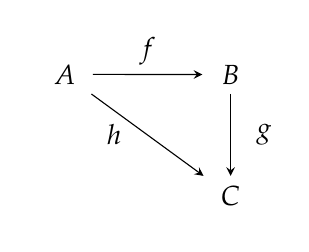
\begin{tikzpicture}
		\matrix (m) [matrix of math nodes,row sep=3em,column sep=4em,minimum width=2em]
		{
			A & B  \\ 
			& C\\};
		\path[-stealth]
		(m-1-1) edge node [above] {$f$} (m-1-2)
		(m-1-1) edge node [left]  {$h~~$} (m-2-2)
		(m-1-2) edge node [right] {$~~g$} (m-2-2);
	\end{tikzpicture}
	\\ 	
	It will be said to \textit{commute} if $h = g\circ f$. The point is that the diagram offers 
	two paths from $A$ to $C$, either by composing to follow $f$ and then $g$, or by 
	following h directly. Commutativity means that the two paths amount to 
	the same thing. A more complex diagram, like the previous one, is said to 
	be commutative when all possible triangles that are parts of the diagram 
	are themselves commutative. This means that any two paths of arrows in 
	the diagram that start at the same object and end at the same object 
	compose to give the same overall arrow. By a \textit{diagram} $D$ in a 
	category $\mathscr C$ we simply mean a collection of $\mathscr C$-objects $d_j, d_k,...$ together 
	with some $\mathscr C$-arrows $g: d_j \to d_k$ between certain of the objects in the 
	diagram. (Possibly more than one arrow between a given pair of objects, 
	possibly none).
	\begin{definition}\label{lim_defn}
		A \textit{cone} for diagram $D$ consists of a $\mathscr C$-object $c$ together with a $\mathscr C$-arrow 
		$c\to d_j$ for each object $f_j$ in $D$, such that
		\newline
		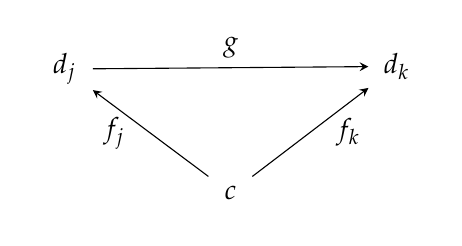
\begin{tikzpicture}
			\matrix (m) [matrix of math nodes,row sep=3em,column sep=4em,minimum width=2em]
			{
				d_j  & & d_k \\ 
				& c  & \\};
			\path[-stealth]
			(m-1-1) edge node [above] {$g$} (m-1-3)
			(m-2-2) edge node [left]  {$f_j~~$} (m-1-1)
			(m-2-2) edge node [right] {$~~f_k$} (m-1-3);
		\end{tikzpicture}
		\\ 	
		commutes, whenever g is an arrow in the diagram $D$. We use the 
		symbolism $\left\{f_j: c\to d_j\right\}$ to denote a cone for $D$. 
		
		
		A \textit{limit} for a diagram $D$ is a $D$-cone $\left\{f_j: c\to d_j\right\}$ with the property that for 
		any other $D$-cone $\left\{f'_j: c'\to d_j\right\}$ there is exactly one arrow $f:c' \to c$ such 
		\newline
		\begin{tikzpicture}
			\matrix (m) [matrix of math nodes,row sep=3em,column sep=4em,minimum width=2em]
			{
				& d_j &  \\ 
				c'	&  & c \\};
			\path[-stealth]
			(m-2-1) edge node [above] {$g$} (m-2-3)
			(m-2-1) edge node [left]  {$f'_j~~$} (m-1-2)
			(m-2-3) edge node [right] {$~~f_j$} (m-1-2);
		\end{tikzpicture}
		\\ 	
		commutes for every object $d_j$ in $D$. 
		This limiting cone, when it exists, is said to have the \textit{universal property} 
		with respect to $D$ -cones.
		A limit for 
		diagram $D$ is unique up to isomorphism.%:- if {ft: —> a\} and {f-:c'—> d;} 			are both limits for D, then the unique commuting arrow f: c'— above is 			iso (its inverse is the unique commuting arrow c-—*c' whose existence 			follows from the fact that {/,': c' —> dj is a limit). 
				% It is universal amongst such cones-any other 		D-cone factors uniquely through it as in the last diagram.		
				
				
			\end{definition} 
			\begin{definition}\label{pull_back_defn}\cite{goldblatt:topoi}
				A \textit{pullback} of a pair $a \xrightarrow{f}c \xleftarrow{g} b$ of $\mathscr C$-arrows with a common codomain 
				is a limit in $\mathscr C$ for the diagram 
				\newline
				\begin{tikzpicture}
					\matrix (m) [matrix of math nodes,row sep=3em,column sep=4em,minimum width=2em]
					{
						& b  \\ 
						a	&  c \\};
					\path[-stealth]
					(m-1-2) edge node [right]  {$g$} (m-2-2)
					(m-2-1) edge node [above] {$f$} (m-2-2);
				\end{tikzpicture}
				\\ 	
				
			\end{definition}
			
			\begin{definition}\label{pullback_defn}\cite{milne:lec}
				For $X$ an object of a category $\mathscr C$, $\mathscr C/X$ denotes the category whose objects are the morphisms $U\to X$ in $\mathscr C$
				and whose arrows are the commutative diagrams 
				\newline
				\begin{tikzcd}
					U \arrow[rr]\arrow[rd] && U'\arrow[ld]\\
					& X &
				\end{tikzcd}
				\\
				A morphism $U \to U'$ making this diagram commute is also referred to as an $X$-\textit{morphism}. The \textit{fibre product} or the \textit{pullback} $U_1\times_X U_2$ of morphisms $\varphi_1: U_1\to X$,  $\varphi_2: U_2\to X$ in $\mathscr C$ is their product in the category $\mathscr C/X$. Thus, there is a commutative diagram 
				\newline
				\begin{tikzcd}
					U_1\times_X U_2 \arrow[d] \arrow[r]
					& U_2 \arrow[d, "\varphi_2"]\\
					U_1\arrow[r, "\varphi_1"]	& X
				\end{tikzcd}
				\\
				\\
				having the obvious universal property. 
				
			\end{definition}
			
			\begin{remark}
				MONIC MONO !!!
			\end{remark}
			\begin{definition}\label{epimorphism_defn}\cite{goldblatt:topoi}
				
				PAGE 39.
				An arrow $f:a\to b$ is epic (right-cancellable) in a category $\mathscr C$ if for any 
				pair of $\mathscr C$-arrows $g, h : b\substack{\to\\\to} c$, the equality $g\circ f = h \circ f$ implies that $g = h$, i.e. 
				whenever a diagram 
				\newline
				\begin{tikzcd}
					a \arrow[d, "f"] \arrow[r, "f"] 
					& b \arrow[d, "g"]\\
					b\arrow[r, "h"]	& c
				\end{tikzcd}
				\\
				\\
				commutes, then $g = h$.
			\end{definition}	
			\begin{definition}\label{initial_ob_defn}\cite{goldblatt:topoi}
				PAGE 43
				
				An object $0_{\mathscr C}$ is \textit{initial} in category $\mathscr C$ if for every $\mathscr C$-object $a$ 
				there is one and only one arrow from $0_{\mathscr C}$ to $a$ in ${\mathscr C}$. 
			\end{definition}
			
			\begin{definition}\label{terminal_ob_defn}\cite{goldblatt:topoi}
				PAGE 44
				An object $1_{\mathscr C}$ is \textit{terminal} in category $\mathscr C$ if for every $\mathscr C$-object $a$ 
				there is one and only one arrow to $0_{\mathscr C}$ to $a$ in ${\mathscr C}$. 
			\end{definition}
			
			\begin{definition}\label{kernel_defn}
				\cite{faith_rmcat}
				If a category $\mathscr C$ has an initial object $0_{\mathscr C}$ then the \textit{kernel} (denoted by $\ker f$ ) of  ${\mathscr C}$-morphism $A \xrightarrow{f} B$ is a limit of the diagram
				\newline
				\begin{tikzcd}
					& 0_{\mathscr C} \arrow[d, ""]\\
					A\arrow[r, "f"]	& X
				\end{tikzcd}
				
			\end{definition}
			\begin{definition}\label{image_defn}\cite{faith_rmcat}
				The \textit{image} of ${\mathscr C}$-morphism $A \xrightarrow{f} B$ (denoted by $\im f$) is an initial object of the category of all monomorphism $I \xrightarrow{\iota} B$ such that there is $\phi_\iota$ with $f = \iota \circ \phi_\iota$ Then the diagram
				\newline
				\begin{tikzcd}
					A \arrow[rr, "f"]\arrow[rd, ""] & & B\\
					& I\arrow[ru, ""] &
				\end{tikzcd}
				\\
				is commutative. %Thus $\im f \to B$ is the minimal monomorphism from the composition.
			\end{definition}
			\begin{definition}\label{exact_sec_defn}\cite{faith_rmcat}
				A sequence of morphisms 
				$$
				...\to A_{j-1}\xrightarrow{f_{j-1}} A_{j}\xrightarrow{f_{j}} A_{j+1}\xrightarrow{f_{j+1}} A_{j+1}\to ...
				$$
				is \textit{exact} if $\ker f_{j+1}= \im f_j$ as subobjects of $A_{j+1}$ for all $j$.
			\end{definition}
			
			
			
			\begin{defn}\label{sets_cat_defn}\cite{johnstone:topos}
				There is the \textit{category  of sets and functions} $\mathscr{S}$. We use the therm \textit{small category} for a category those morphisms form a set. If $\mathscr C$ is a small category, we write $\mathscr{S}^{\mathscr{C}^{\mathrm{op}}}$ for the category of \textit{presheaves}, i.e. contravariant functors from $\mathscr{C}$ to $\mathscr{S}$; among the objects of $\mathscr{S}^{\mathscr{C}^{\mathrm{op}}}$, we have the \textit{representable} functors $h_U$, where $U$ is an object of $\mathscr C$, defined by $h_U\left( V\right) \bydef \Hom_{\mathscr{C}}\left( V, U\right)$; we shall also write $h^U$ for the covariant representable  functor $\Hom_{\mathscr{C}}\left( U, -\right)$.
			\end{defn}
			\begin{lemma}\label{repr_func_lem}\cite{johnstone:topos}
				For objects $U$, $X$ of $\mathscr{C}$ and $\mathscr{S}^{\mathscr{C}^{\mathrm{op}}}$ respectively there is a bijection (natural in both variables) between morphisms $h_U \to X$ in $\mathscr{S}^{\mathscr{C}^{\mathrm{op}}}$ and elements of the set $X\left(U \right)$. 
			\end{lemma}
			\begin{lemma}\label{to_set_lem}\cite{johnstone:topos}
				Any object of $\mathscr{S}^{\mathscr{C}^{\mathrm{op}}}$ can be expressed as a colimit of a diagram whose vertices are representable functors.
			\end{lemma}
			
			\begin{definition}
				\label{(co)complete_defn}A category $\mathbf{C}$ is called \textit{complete}
				if it admits small limits, and \textbf{cocomplete} if it admits small
				colimits.
			\end{definition}
			
			
			\begin{proposition}\cite{borce_cat}\label{fin_lim_prop}
				%Proposition 2.8.2. 
				For a category $\mathscr C$ 
				the following are equivalent:
				\begin{enumerate}
					\item $\mathscr C$
					is finitely complete; 
					
					\item $\mathscr C$
					has a terminal object, binary products and equalizers;
					
					\item $\mathscr C$
					has a terminal object and pullbacks.
					
					
				\end{enumerate}
			\end{proposition}
			
			\begin{definition}\label{injective_object_defn}\cite{topos:intro}
				In any category $\mathscr C$, an object $K$ is said to be \textit{injective} when for
				every monomorphism $m: S \to B$ in $\mathscr C$ every $f: S\to K$ can be extended
				to $g: B \to K$ with $g\circ m = f$, as in the diagram
				\newline
				\begin{tikzcd}
					S \arrow[r, "m"]\arrow[d, "f"] & B\arrow[ld, "g"]\\
					K &
				\end{tikzcd}
				\\
				Equivalently, this states that for each monomorphism $m: S \to B$ the
				induced map
				\bean
				m^*: \Hom( B, K) \to \Hom( S, K) 
				\eean
				is onto. 	
			\end{definition}
			\subsection{Functors}
			\begin{definition}\label{functor_defn}\cite{goldblatt:topoi}
				A \textit{functor} $F$ from category $\mathscr{C}$ to category $\mathscr{D}$ is a function that assigns 
				\begin{enumerate}
					\item [(i)]
					to each $\mathscr{C}$-object $a$, a $\mathscr{D}$-object $F(a)$; 
					\item[(ii)] to each $\mathscr{C}$-arrow $f:a \to b$ a $\mathscr{D}$-arrow $F(f): F(a) \to F(b)$, 
					such that 
					\begin{enumerate}
						\item[(a)]  $F\left(\mathbb 1_a\right) = \mathbb 1_{F\left(a\right)}$ for all  $\mathscr{C}$-objects $a$, i.e. the identity arrow on $a$ is assigned 
						the identity on $F\left(a\right)$,
						\item[(b)]  $F\left(g\circ f\right)=F\left(g\right)\circ F\left( f\right) $, whenever $g \circ f$ is defined. 
						This last condition states that the $F$-image of a composite of two arrows 
						is the composite of their $F$-images.
					\end{enumerate}
					
					
				\end{enumerate}
				We write $F:\mathscr{C}\to \mathscr{D}$ or  $\mathscr{C}\xrightarrow{F} \mathscr{D}$ to indicate that $F$ is a 
				functor from $
				\mathscr{C}$ to $\mathscr{D}$. Briefly then a functor is a transformation that 
				"preserves" dom's, cod's, identities and composites. 
			\end{definition}
			If $a$ and $b$ are  $\mathscr{C}$-objects then a functor $\mathscr{C}\xrightarrow{F} \mathscr{D}$ yields a map
			\be\label{f_ab_funct_eqn}
			F_{a,b}:\mathscr{C}\left(a, b \right)  \to \mathscr{D}\left( F\left(a\right), F\left(b\right)\right)  
			\ee
			(cf. Notation \ref{category_not}).
			\begin{definition}\label{funct_full_faithfull_defn}\cite{bass}
				A functor $\mathscr{C}\xrightarrow{F} \mathscr{D}$ is said to be \textit{faithful} (resp. \textit{full}) if the given by \eqref{f_ab_funct_eqn} map is injective (resp. surjective).
			\end{definition}
			\begin{defn}\label{functor_contravariant_defn}\cite{goldblatt:topoi}
				A \textit{contravariant} functor is one that reverses direction by mapping domains 
				to codomains and vice versa. 
				Thus $\mathscr{C}\xrightarrow{F} \mathscr{D}$ is a contravariant functor if it assigns to $f: a\to b$ an 
				arrow $F(f):F(b)\to F(a)$, so that $F\left(\mathbb{1}_a\right)= \mathbb{1}_{F(a)}$ as before, but now 
				$$
				F\left( g\circ f\right) = F\left( f\right)\circ  F\left( g\right). 
				$$
			\end{defn}
			
			
			\begin{definition}\label{exact_functor_defn}\cite{goldblatt:topoi}
				A left/right exact functor is a functor that preserves finite limits/finite colimits.
			\end{definition}
			\subsection{Natural transformations}\label{natural_transformation_sec}
			\paragraph{}
			Here I follow to \cite{goldblatt:topoi}.
			Given two categories $\mathscr C$ and $\mathscr D$ we are going to construct a category, 
			denoted $\mathrm{Funct}\left(\mathscr C, \mathscr D\right)$, or $\mathscr D^{\mathscr C}$, whose objects are the functors from $\mathscr C$ to $\mathscr D$. 
			We need a definition of arrow from one functor to another. Let 
			$F: \mathscr C\to \mathscr D$ and $G: \mathscr C\to \mathscr D$ be two functors. For any $\mathscr C$-object $a$ we define a $\mathscr D$-arrow $\tau_a : F\left(a\right)\to  G\left(a\right)$. We require that each  $\mathscr C$-arrow $f: a \to b$  gives rise to a diagram 
			\\
			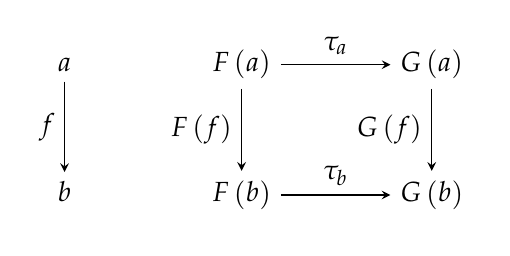
\begin{tikzpicture}
				\matrix (m) [matrix of math nodes,row sep=3em,column sep=4em,minimum width=2em]
				{
					a	& F\left(a \right)  &   G\left(a \right)\\ 
					b	& F\left(b \right)  &   G\left(b \right) \\};
				\path[-stealth]
				(m-1-1) edge node [left]  {$f$} (m-2-1)
				(m-1-2) edge node [above] {$\tau_a$} (m-1-3)
				(m-2-2) edge node [above]  {$\tau_b$} (m-2-3)
				(m-1-2) edge node [left]  {$F\left( f \right)$} (m-2-2)
				(m-1-3) edge node [left]  {$G\left( f \right)$} (m-2-3);
			\end{tikzpicture}
			\\ 	
			that commutes.
			%a F(a) Ta > G(a) Ftf)  F(b) T"  G(b) that commutes. Thus  and provide a categorical way of turning the F-picture of f:a-*b into its G-picture. 
			In summary then, a \textit{natural transformation} from functor $F: \mathscr C\to \mathscr D$ and $G: \mathscr C\to \mathscr D$  to functor $F: \mathscr C\to \mathscr D$ and $G: \mathscr C\to \mathscr D$  is an assignment $\tau$ that provides, for each $\mathscr C$-object $\mathscr D$-arrow $\tau_a :F(a) \to G(a)$, such that for any $\mathscr C$-arrow $f:a\to b$, the above diagram commutes in $\mathscr D$, i.e. $\tau_b \circ F(f)= G(f)\circ \tau_a$. We use the symbolism $\tau: F\to G$, or $F \xrightarrow{\tau}G$, to denote that $\tau$ is a natural transformation from $F$ to $G$. The arrows $\tau_a$ are called the \textit{components} of $a$. Now if each component $\tau_a$ of $a$ is an iso arrow in $\mathscr D$ then  case we call $\tau$ a \textit{natural isomorphism}. Each $\tau_a: F(a)\to G(a)$ then has an inverse $\tau_a^{-1}: G(a) \to F(a)$, and these $\tau^{-1}_a$'s form the components of a natural isomorphism $\tau^{-1}: G \to F$. We denote natural isomorphism by $\tau: F \cong G$. 
			\begin{example}
				The identity natural transformation $\mathbb{1}_F :F\to F$ assigns to each object $a$, the identity arrow $\mathbb{1}_{F(a)}:F(a)\to F(a)$. This is clearly a natural isomorphism. 
			\end{example}
			
			\begin{definition}\label{category_equivalence_definition}\cite{goldblatt:topoi}
				A functor $F: \mathscr C\to  \mathscr D$ is called an \textit{equivalence of categories} if there 
				is a functor $G: \mathscr D\to  \mathscr C$ such that there are natural isomorphisms $\tau : 1_{\mathscr C} \cong G \circ F$, and $\sigma : 1_{\mathscr D} \cong F \circ G$, from the identity functor on ${\mathscr C}$ to $ G \circ F$, and 
				from the identity functor on ${\mathscr D}$ to $ F \circ G$.
				
				Categories $\mathscr C$ and $\mathscr D$ are \textit{equivalent},  $\mathscr C$ and $\mathscr D$ when there exists an equivalence $F: \mathscr C\to  \mathscr D$ .
			\end{definition}
			
			
			
			
			
			%We assume that reader is familiar with the notions of \textit{limit} and \text{colimit}.
			
			
			\subsection{Adjoint functors}\label{adjoint_functor_sec}
			\paragraph*{}
			
			If both $\mathscr C$ and $\mathscr D$ are categories then a pair of functors $\mathscr C \substack{ \xrightarrow{F}\\\xleftarrow[G]{}}\mathscr D$ are \textit{adjoint functors} if for any $\mathscr C$-object $A$ and $\mathscr D$-object $B$ there is a natural bijection
			$$
			\Hom_{\mathscr D}\left(F\left(A \right), B  \right) \cong \Hom_{\mathscr C}\left(A, G\left(B \right)  \right).
			$$
			A pair of {adjoint functors} can be defined via counit–unit adjunction, i.e. there are natural transformations
			\bean
			\eps : FG \to 1_{\mathscr C},\\
			\eta : 1_{\mathscr  D} \to  GF 
			\eean
			respectively called the \textit{counit} and the \textit{unit} of the adjunction (terminology from universal algebra), such that the compositions
			\be\label{id_thens_eqn}
			\begin{split}
				F{\xrightarrow {\;F\eta \;}}FGF{\xrightarrow {\;\varepsilon F\,}}F,\\
				G{\xrightarrow {\;\eta G\;}}GFG{\xrightarrow {\;G\varepsilon \,}}G
			\end{split}
			\ee
			are the identity transformations $1_F$ and $1_G$ on $F$ and $G$ respectively. $F$ is said to be \textit{left adjoint} $G$, and $G$ is \textit{right adjoint} $F$.
				
			
						
						
					\end{appendices}
					

		
 \end{document}